\chapter{Kiến Thức Nền Tảng}
\ifpdf
    \graphicspath{{Chapter2/Chapter2Figs/PNG/}{Chapter2/Chapter2Figs/PDF/}{Chapter2/Chapter2Figs/}}
\else
    \graphicspath{{Chapter2/Chapter2Figs/EPS/}{Chapter2/Chapter2Figs/}}
\fi

\begin{quote}

Trong chương này, chúng tôi sẽ trình bày những kiến thức nền tảng trên ba chủ đề bao gồm mạng nơ-ron hồi quy, mô hình ngôn ngữ nơ-ron và mô hình dịch máy nơ-ron. Mạng nơ-ron hồi quy (RNN) là xương sống của dịch máy nơ-ron. Nó được sử dụng để làm cả bộ mã hóa lẫn bộ giải mã. Ứng với mỗi vai trò, RNN sẽ có một thiết kế riêng. Một phiên bản cải tiến của RNN là \textit{Long short-term memory} cũng được chúng tôi trình bày, phiên bản này giúp cho việc huấn luyện RNN trở nên dễ dàng hơn. Sau đó, dựa trên những kiến thức về mạng nơ-ron hồi quy, chúng tôi nói về khái niệm \textit{mô hình ngôn ngữ} với chức năng tạo ra từ trong bộ giải mã, là bước quan trọng trong dịch máy nơ-ron. Cuối cùng, chúng tôi cũng trình bày về mô hình dịch máy nơ-ron theo kiến trúc bộ mã hóa - bộ giải mã với RNN và mô hình ngôn ngữ hồi quy là những thành phần nền tảng.

\end{quote}
\section{Mạng nơ-ron hồi quy (Recurrent neural network)}

Trong tự nhiên, dữ liệu không phải lúc nào cũng được sinh ra một cách ngẫu nhiên. Trong một số trường hợp, chúng được sinh ra theo một thứ tự. Xét trong dữ liệu văn bản, ví dụ ta cần điền vào chỗ trống cho câu sau \textit{"Paris là thủ đô của nước \_\_"}. Dễ biết được rằng chỉ có duy nhất một từ phù hợp cho chỗ trống này, đó là \textit{"Pháp"}. Điều này có nghĩa là mỗi từ trong một câu không được tạo ra ngẫu nhiên mà nó được tạo ra dựa trên một liên hệ với những từ đứng trước nó. Các loại dữ liệu khác như những khung hình trong một bộ phim hoặc các đoạn âm thanh trong một bản nhạc cũng có tính chất tương tự. Những loại dữ liệu mang thứ tự này được gọi chung là dữ liệu chuỗi (sequential data).

Trong quá khứ, một số mô hình xử lý dữ liệu chuỗi bằng cách giả định rằng đầu vào hiện tại có liên hệ với một số lượng xác định đầu vào trước đó, nhiều mô hình tạo ra một cửa sổ trượt để nối mỗi đầu vào hiện tại với một số lượng đầu vào trước đó nhằm tạo ra sự mô phỏng về tính phụ thuộc. Cách tiếp cận này đã được sử dụng cho mô hình \textit{Deep belief network} trong xử lý tiếng nói \cite{massetal2012}. Nhược điểm của những cách làm này là ta phải xác định trước kích thước của cửa sổ. Một mô hình với kích thước cửa sổ với chiều dài bằng 6 không thể nào quyết định được từ tiếp theo trong câu \textit{"Hổ là loài động vật ăn \_\_"} sẽ là \textit{"thịt"} hay \textit{"cỏ"}. Trong ví dụ này, từ tiếp theo của câu phụ thuộc mật thiết vào từ \textit{"Hổ"} cách nó đúng 6 từ. Trên thực tế, có rất nhiều câu đòi hỏi sự phụ thuộc với nhiều từ xa hơn trước đó. Ta gọi những sự phụ thuộc kiểu như vậy là những \textit{phụ thuộc dài hạn} (long term dependency). 

\textit{Mạng nơ-ron hồi quy} (recurrent neural network) \cite{elman1990} gọi tắt là \textit{RNN} là một nhánh của nạng nơ-ron nhân tạo được thiết kế đặc biệt cho việc mô hình hóa dữ liệu chuỗi. Khác với những mô hình đã đề cập giả định sự phụ thuộc chỉ xảy ra trong một vùng có chiều dài cố định. RNN, trên lý thuyết, có khả năng nắm bắt được các phụ thuộc dài hạn với chiều dài bất kỳ. Để làm được điều đó, trong quá trình học, RNN lưu giữ những thông tin cần thiết cho các phụ thuộc dài hạn bằng một vec-tơ được gọi là \textit{trạng thái ẩn}.

Xét một chuỗi đầu vào $x={x_1,x_2,...,x_n}$. Ta gọi $h_t$ là trạng thái ẩn tại \textit{bước thời gian} (timestep) $t$, là lúc một mẫu dữ liệu $x_t$ được đưa vào RNN để xử lý. Trạng thái ẩn $h_t$ sẽ được tính toán dựa trên mẫu dữ liệu hiện tại $x_t$ và trạng thái ẩn trước đó $h_{t-1}$. Có thể thể hiện $h_t$ như một hàm hồi quy với tham số là đầu vào hiện tại và chính nó ở thời điểm trước đó:
\begin{equation} \label{basicRnnEquation}
	h_t = f \left(h_{t-1}, x_t \right)
\end{equation}
trong đó hàm $f$ là một ánh xạ phi tuyến. Có thể hình dung $h_t$ như một đại diện cho những đầu vào mà nó đã xử lý từ thời điểm ban đầu cho đến thời điểm $t$. Nói một cách khác, RNN sử dụng trạng thái ẩn như một dạng bộ nhớ để lưu giữ thông tin từ một chuỗi. Hình \ref{fig_rnn_loop} thể hiện định nghĩa hồi quy của RNN.

\begin{figure}
	\centering
	\includegraphics[width=0.25\textwidth]{rnn_loop}
	\caption[Mô hình RNN với kết nối vòng]{Mô hình RNN đơn giản với kết nối vòng, \textbf{$h$} được xem như bộ nhớ được luân chuyển trong RNN. Chú ý rằng đường nét đứt ở đầu ra thể hiện rằng tại một thời điểm $t$, RNN có thể có hoặc không có một đầu ra.}
	\label{fig_rnn_loop}
\end{figure}
Thông thường, hàm $f$ là một hàm phi tuyến như hàm \textit{$\sigma$} hay hàm \textit{$\tanh$}. Xét một RNN với công thức cụ thể như sau:
\begin{equation} \label{rnnWithTanh}
	h_t = \phi \left(W_{xh} x_t + W_{hh}h_{t-1} + b_h \right)
\end{equation}
Trong đó:
\begin{itemize}
	\item[•] $\phi$ là một hàm kích hoạt (ví dụ: sigmoid, tanh hay ReLU).
	\item[•] $h_{t} \in \mathbb{R}^n$ là trạng thái ẩn tại bước thời gian hiện tại.
	\item[•] $x_t \in \mathbb{R}^m$ là đầu vào hiện tại.
	\item[•] $h_{t-1} \in \mathbb{R}^n$ là trạng thái ẩn tại bước thời gian trước đó.
	\item[•] $W_{xh} \in \mathbb{R}^{m \times n}, W_{hh} \in \mathbb{R}^{n \times n}$ và $b_h \in \mathbb{R}^n$ lần lượt là hai ma trận trọng số và vec-tơ "bias".
\end{itemize}

Ma trận $W_{xh}$ là làm nhiệm vụ kết nối giữa đầu vào và trạng thái ẩn, $W_{hh}$ kết nối trạng thái ẩn với chính nó trong các bước thời gian liền kề. Vec-tơ $b_h$ dùng để điều chỉnh giá trị của $h_t$. Tại thời điểm bắt đầu, trạng thái ẩn $h_0$ có thể được khởi tạo bằng 0 hoặc là một vector chứa tri thức có sẵn như trường hợp của bộ giải mã như chúng tôi đã đề cập trong chương 1.

Tại mỗi bước thời gian $t$, tùy vào mục tiêu cụ thể của quá trình học mà RNN có thể có thêm một đầu ra $y_t$. Trong ngữ cảnh bài toán dịch máy nơ-ron, đầu ra của RNN trong quá trình giải mã chính là một từ trong ngôn ngữ đích hay nói chung là một đầu ra dạng rời rạc. Với mục tiêu đó, đầu ra dự đoán của RNN $\hat{y}_t$ sẽ có dạng là một phần phối xác suất trên tập các các lớp ở đầu ra. Phân phối này nhằm dự đoán vị trí xuất hiện của $\hat{y}_t$.
%\begin{equation} \label{rnnOuputSoftmax}
%	s_t = W_{hy}h_t + b_y
%\end{equation} 
\begin{equation} \label{rnnOuputSoftmaxDistribution}
	\hat{y}_t = \softmax(W_{hy}h_t + b_y)
\end{equation}
Trong đó:
\begin{itemize}
	\item[•] $\softmax$ là một hàm kích hoạt với $\softmax(v_j) = \frac{e^{v_j}}{\sum_{k=1}^{K}e^{v_k}}$, $j = 1,...,K$, $K$ là độ dài của vec-tơ $v$.
	\item[•] $h_{t} \in \mathbb{R}^n$ là trạng thái ẩn tại bước thời gian hiện tại.
	\item[•] $W_{hy} \in \mathbb{R}^{L \times n}$ và $b_y \in \mathbb{R}^L$ lần lượt là hai ma trận trọng số và vec-tơ "bias". $L$ là số lượng lớp cần phân biệt ở đầu ra.
\end{itemize}

Trong công thức trên, hàm $\softmax$ đóng vai trò là một hàm chuẩn hóa để $\hat{y}_t$ thể hiện một phân phối xác suất trên các lớp ở đầu ra. Ma trận $W_{hy}$ kết nối đầu ra với trạng thái ẩn, $b_y$ dùng để điều chỉnh giá trị của kết quả tính toán trước khi đưa qua hàm $\softmax$.

\begin{figure}
	\centering
	\includegraphics[width=0.85\textwidth]{rnn_unrolled}
	\caption[Mô hình RNN dạng dàn trải]{Mô hình RNN được dàn trải (unrolled), ví dụ trong 4 bước thời gian.}
	\label{fig_rnn_unrolled}
\end{figure}

Để ý rằng các ma trận trọng số $W_{xh}$, $W_{hh}$, $W_{hy}$ và các vector bias $b_h$, $b_y$ là các tham số học của mô hình và chúng là duy nhất. Có nghĩa là khi những tham số này được học, bất kỳ một đầu vào nào cũng đều sử dụng chung một bộ tham số. Điều này chính là sự chia sẻ tham số (parameters sharing) trong mạng nơ-ron hồi quy. Chia sẻ tham số khiến cho mô hình học dễ dàng hơn, nó giúp cho RNN có thể xử lý chuỗi đầu vào với độ dài bất kỳ mà không làm tăng độ phức tạp của mô hình. Quan trọng hơn, nó giúp ích cho việc tổng quát hóa. Đây chính là điểm đặc biệt của RNN so với mạng nơ-ron truyền thẳng.

Với một số lượng hữu hạn các bước thời gian, mô hình RNN trên hình \ref{fig_rnn_loop} có thể được dàn trải ra (unrolled). Dạng dàn trải này được miêu tả trực quan như trên hình \ref{fig_rnn_unrolled}. Với cách thể hiện này, RNN có thể được hiểu như là một mạng nơ-ron sâu với mỗi bước thời gian là một mạng nơ-ron một tầng ẩn và các tham số học được chia sẻ giữa các mạng nơ-ron đó. Dạng dàn trải cũng thể hiện rằng RNN có thể được huấn luyện qua nhiều bước thời gian bằng thuật toán lan truyền ngược (backpropagation). Thuật toán này được gọi là "Backpropagation through time" (BPTT) \cite{werbos1990}. Thực chất đây là chỉ thuật toán “Backpropagation” khi áp dụng cho RNN dưới dạng dàn trải để tính "gradient" cho các tham số ở từng bước thời gian. Hầu hết cả các mạng nơ-ron hồi quy phổ biến ngày nay đều áp dụng thuật toán này vì tính đơn giản và hiệu quả của nó.

\subsection{Huấn luyện mạng nơ-ron hồi quy}

Xét một chuỗi đầu vào $x={x_1,x_2,...,x_n}$ với đầu ra tương ứng $y={y_1,y_2,...,y_n}$. Trong quá trình lan truyền tiến, tại mỗi bước thời gian $t$ ứng mẫu dữ liệu $(x_t, y_t)$, công thức tính toán đầu ra dự đoán có dạng:
\begin{equation} \label{rnnForwardProp1}
	h_t = \phi \left(W_{xh} x_t + W_{hh}h_{t-1} + b_h \right) 
\end{equation}
\begin{equation} \label{rnnForwardProp2}
	s_t = W_{hy} h_t + b_y 
\end{equation}
\begin{equation} \label{rnnForwardProp3}
	\hat{y}_t = softmax (s_t) 
\end{equation}
Ta xác định hàm độ lỗi độ lỗi giữa đầu ra dự đoán $\hat{y}_t$ và đầu ra thật sự $y_t$. Gọi $V$ là số lượng lớp của $y$, lúc này có thể thấy $\hat{y}_t$ là một vec-tơ phân phối xác suất có độ dài $V$. Để so sánh với $\hat{y}_t$, $y_t$ được chuẩn hóa thành một vec-tơ dạng "one hot" có nghĩa là một vec-tơ với độ dài $V$ có giá trị bằng 0 trừ vị trí ứng với lớp của $y_t$ có giá trị 1. Như vậy để so sánh hai phân phối xác suất $y$ và $\hat{y}$ ta sử dụng hàm độ lỗi \textit{negative log-likelihood} hay còn gọi là \textit{cross entropy}:
\begin{equation} \label{errorOfAnExample}
	E_t = -y_t\log(\hat{y}_t)
\end{equation}
trong đó $E_t$ là độ lỗi tại một bước thời gian $t$. Độ lỗi của toàn bộ quá trình học $E$ là tổng của độ lỗi tại của tất cả các bước thời gian.
\begin{equation} \label{errorOfAll}
	E = \sum_{t}E_t = - \sum_{t}y_t\log(\hat{y}_t) 
\end{equation}

% TODO: tai sao su dung mini batch
Mục tiêu của việc học là cực tiểu hóa độ lỗi tổng hợp $E$. Thuật toán "backpropagation" với \textit{gradient descent} sẽ được áp dụng để huấn luyện RNN. Trên thực tế, người ta sẽ sử dụng một phiên bản của "gradient descent" là "mini-batch gradient descent" cho việc huấn luyện. Tập dữ liệu ban đầu sẽ được chia thành nhiều "mini-batch", mỗi "mini-batch" là một tập con với số lượng khoảng vài chục đến vài trăm mẫu thuộc tập dữ liệu ban đầu. Với mỗi lần duyệt (iteration), việc tính toán gradient để cập nhật các tham số học của mô hình được thực hiện lần lượt trên tất cả các mini-batch này.

Ta cần tìm bộ tham số $\theta = \left(W_{hy},W_{hh},W_{xh},b_y,b_h \right)$ sao cho cực tiểu hóa hàm độ lỗi $E$. Theo thuật toán "gradient descent", bộ tham số được cập nhật theo công thức:
\begin{equation} \label{gradientDescentWithTheta}
	\theta \leftarrow \theta - \eta \frac{\partial{E} }{\partial{\theta}}
\end{equation}

% TODO: Bo sung cho nay
Ở đây, $\frac{\partial{E} }{\partial{\theta}}$ là "gradient" của hàm độ lỗi ứng với các tham số của mô hình. $\eta$ được gọi là hệ số học (learning rate) là một siêu tham số quyết định rằng $\theta$ nên thay đổi nhiều bao nhiêu khi "gradient" ứng với tham số thay đổi. Trong phần dưới đây, chúng tôi sẽ trình bày việc tính toán "gradient" của hàm độ lỗi theo bộ tham số học $\theta = \left(W_{hy},W_{hh},W_{xh},b_y,b_h \right)$.

\subsubsection{Gradient theo $W_{hy}$ và $b_y$}
Bởi vì $W_{hy}$ và $b_y$ chỉ hiện diện trong hàm $\hat{y}$. Với $s_t = W_{hy} h_t + b_y$ và $\hat{y}_t = softmax(s_t)$, sử dụng công thức nhân trong tính đạo hàm ta được:
\begin{equation} \label{gradientWRTSt1}
	\frac{\partial{E_t}}{\partial{W_{hy}}} = \frac{\partial{E_t}}{\partial{\hat{y}}} \frac{\partial{\hat{y}}}{\partial{s_t}} \frac{\partial{s_t}}{\partial{W_{hy}}}
\end{equation}

Từ công thức \ref{errorOfAnExample} ta có:
\begin{equation} \label{gradientWRTSt2}
	\frac{\partial{E_t}}{\partial{\hat{y}}} = -\frac{y_t}{\hat{y}_t}
\end{equation}

Hàm $\hat{y}$ là một hàm $\softmax$ nên nó có đạo hàm:
\begin{equation} \label{gradientWRTSt3}
	\frac{\partial \hat{y}_{t}}{\partial s_{t}}=\left\{
		\begin{array}{lr}
			-\hat{y}_{t_k}\hat{y}_{t_l}, & k\neq l \\
			\hat{y}_{t_k}\left(1-\hat{y}_{t_k}\right), & k=l
		\end{array}
	\right..
\end{equation}

Kết hợp \ref{gradientWRTSt2} và \ref{gradientWRTSt3} ta có được:
\begin{subequations} \label{gradientWRTSt4}
\begin{align}
-\frac{y_{t_l}}{\hat{y}_{t_l}}\hat{y}_{t_l}\left(1-\hat{y}_{t_l}\right)+\sum_{k\ne l}{}\left(-\frac{y_{t_k}}{\hat{y}_{t_k}}\right)\left(-\hat{y}_{t_k}\hat{y}_{t_l}\right) 
&= -y_{t_l}+y_{t_l}\hat{y}_{t_l}+\sum_{k\ne l}{}y_{t_k}\hat{y}_{t_l} \\
&= -y_{t_l} + \hat{y}_{t_l}\sum_{k}{}y_{t_k}.
\end{align}
\end{subequations}

Lưu ý rằng $y_t$ là "one-hot" vec-tơ nên tổng trong công thức trên bằng 1, cho nên:

\begin{equation} \label{gradientWRTSt5}
	\frac{\partial{E_t}}{\partial{s_t}} = \hat{y}_t - y_t
\end{equation}

Bởi vì $W_{hy}$ được chia sẻ trên toàn bộ chuỗi, do đó đạo hàm hàm độ lỗi tổng hợp $E$ theo $W_{hy}$ sẽ là tổng đạo hàm của các $E_t$ theo $W_{hy}$. Từ công thức \ref{gradientWRTSt5} ta có được:
\begin{equation} \label{gradientWRTSt6}
	\frac{\partial{E}}{\partial{W_{hy}}} = \sum_{t} \frac{\partial{E_t}}{\partial{s_t}} \frac{\partial{s_t}}{\partial{W_{hy}}} = \sum_{t} \left(\hat{y}_t - y_t \right) \otimes h_t
\end{equation}

trong đó $\otimes$ là "outer-product" của hai vec-tơ.

Tương tự với đạo hàm của $E$ theo $b_y$, ta cũng có:
\begin{equation} \label{gradientWRTSt7}
	\frac{\partial{E}}{\partial{b_{y}}} = \sum_{t} \frac{\partial{E_t}}{\partial{s_t}} \frac{\partial{s_t}}{\partial{b_{y}}} = \sum_{t} \hat{y}_t - y_t
\end{equation}

\subsubsection{Gradient theo $W_{hh}$, $W_{xh}$ và $b_h$}

Tham số $W_{hh}$ tồn tại ở cả trạng thái ẩn $h_t$ và đầu ra dự đoán $\hat{y}_t$, để tính "gradient" theo $W_{hh}$. Chúng ta cũng để ý rằng $\hat{y}_t$ cũng dựa trên $W_{hh}$ trực tiếp và gián tiếp (thông qua $h_{t-1}$). Đặt $p_t = W_{hx}x_t + W_{hh}h_{t-1}$ và $h_t = \tanh(p_t)$:
\begin{equation} \label{gradientWRTSt8}
	\frac{\partial{E_t}}{\partial{W_{hh}}} = \frac{\partial{E_t}}{\partial{\hat{y}}} \frac{\partial{\hat{y}}}{\partial{s_t}} \frac{\partial{s_t}}{\partial{h_t}} \frac{\partial{h_t}}{\partial{W_{hh}}}
\end{equation}

Trong công thức trên, ta đã biết $\frac{\partial{E_t}}{\partial{\hat{y}}}$ và $\frac{\partial{\hat{y}}}{\partial{s_t}}$ trong phần trước, công thức tính $\frac{\partial{s_t}}{\partial{h_t}}$ khá đơn giản:
\begin{equation} \label{gradientWRTSt9}
	\frac{\partial{s_t}}{\partial{h_t}} = W_{hy}
\end{equation}

Cuối cùng, để tính được $\frac{\partial{h_t}}{\partial{W_{hh}}}$ ta có quan sát rằng có một sự phụ thuộc giữa $h_t$ và $W_{hh}$ thông qua trạng thái ẩn trước đó $h_{t-1}$. Ta biết rằng nếu $f(x,y)$ với $x, y \in \mathbb{R}^N$, giả sử $x,y$ là những hàm số của $r$ sao cho $x = x(r); y = y(r)$ thì ta có:
  \begin{equation} \label{gradientWRTSt10}
	\frac{\partial{f}}{\partial{r}} = \frac{\partial{f}}{\partial{x}}\frac{\partial{x}}{\partial{r}} + \frac{\partial{f}}{\partial{y}}\frac{\partial{y}}{\partial{r}}
\end{equation}

Áp dụng công thức trên để tính $\frac{\partial{h_t}}{\partial{W_{hh}}}$ ta được:
\begin{equation} \label{gradientWRTSt11}
	\frac{\partial{h_t}}{\partial{W_{hh}}} = \frac{\partial{h_t}}{\partial{W_{hh}}} + \frac{\partial{h_t}}{\partial{h_{t-1}}} \frac{\partial{h_{t-1}}}{\partial{W_{hh}}}
\end{equation}

Tuy nhiên, ta có thể áp dụng công thức trên một lần nữa với $\frac{\partial{h_{t-1}}}{\partial{W_{hh}}}$:
\begin{equation} \label{gradientWRTSt12}
	\frac{\partial{h_t}}{\partial{W_{hh}}} = \frac{\partial{h_t}}{\partial{W_{hh}}} + \frac{\partial{h_t}}{\partial{h_{t-1}}} \frac{\partial{h_{t-1}}}{\partial{W_{hh}}} + \frac{\partial{h_t}}{\partial{h_{t-1}}} \frac{\partial{h_{t-1}}}{\partial{h_{t-2}}} \frac{\partial{h_{t-2}}}{\partial{W_{hh}}}
\end{equation}

Quá trình này tiếp tục cho đến khi chúng kết thúc ở $h_0$ là trạng thái ẩn khởi tạo. Có thể thấy 
\begin{equation} \label{gradientWRTSt122}
\frac{\partial{h_t}}{\partial{h_{t-1}}} \frac{\partial{h_{t-1}}}{\partial{h_{t-2}}} \frac{\partial{h_{t-2}}}{\partial{W_{hh}}} = \frac{\partial{h_t}}{\partial{h_{t-2}}} \frac{\partial{h_{t-2}}}{\partial{W_{hh}}}
\end{equation}
và:
\begin{equation} \label{gradientWRTSt123}
\frac{\partial{h_t}}{\partial{W_{hh}}} = \frac{\partial{h_t}}{\partial{h_{t}}} \frac{\partial{h_t}}{\partial{W_{hh}}}
\end{equation}

Như vậy, có thể rút gọn \ref{gradientWRTSt12} thành một công thức duy nhất:
\begin{equation} \label{gradientWRTSt13}
	\frac{\partial{h_t}}{\partial{W_{hh}}} = \sum_{r=0}^{t} \frac{\partial{h_t}}{\partial{h_r}} \frac{\partial{h_r}}{\partial{W_{hh}}}
\end{equation}

Kết hợp các công thức từ \ref{gradientWRTSt8} suy ra:
\begin{equation} \label{gradientWRTSt14}
	\frac{\partial{E_t}}{\partial{W_{hh}}} = (\hat{y}_t - y_t) W_{hy} \sum_{r=0}^{t} \frac{\partial{h_t}}{\partial{h_r}} \frac{\partial{h_r}}{\partial{W_{hh}}}
\end{equation}

Đạo hàm hàm độ lỗi tổng hợp $E$ theo $W_{hh}$ sẽ là tổng đạo hàm của các $E_t$ theo $W_{hh}$
\begin{equation} \label{gradientWRTSt15}
	\frac{\partial{E}}{\partial{W_{hh}}} = \sum_{t=0}^{T} \sum_{r=0}^{t} (\hat{y}_t - y_t) W_{hy}\frac{\partial{h_t}}{\partial{h_r}} \frac{\partial{h_r}}{\partial{W_{hh}}}
\end{equation}

Cũng giống như $W_{hh}$, trong công thức tính $h_t$, $W_{hh}$ cũng có liên hệ với $h_t$ một cách trực tiếp và với $h_{t-1}$ một cách gián tiếp. Ta có:
\begin{equation} \label{gradientWRTSt16}
	\frac{\partial{E_t}}{\partial{W_{xh}}} = \frac{\partial{E_t}}{\partial{\hat{y}}} \frac{\partial{\hat{y}}}{\partial{s_t}} \frac{\partial{s_t}}{\partial{h_t}} \frac{\partial{h_t}}{\partial{W_{hx}}}
\end{equation}

Ta chỉ cần tính $\frac{\partial{h_t}}{\partial{W_{hx}}}$, theo cách tương tự như đã làm với $W_{hh}$ ,ta được:
\begin{equation} \label{gradientWRTSt17}
	\frac{\partial{h_t}}{\partial{W_{xh}}} = \sum_{r=0}^{t} \frac{\partial{h_t}}{\partial{h_r}} \frac{\partial{h_r}}{\partial{W_{xh}}}
\end{equation}

Như vậy cuối cùng ta được:
\begin{equation} \label{gradientWRTSt18}
	\frac{\partial{E_t}}{\partial{W_{hh}}} = (\hat{y}_t - y_t) W_{hy} \sum_{r=0}^{t} \frac{\partial{h_t}}{\partial{h_r}} \frac{\partial{h_r}}{\partial{W_{xh}}}
\end{equation}

Điểm khác biệt giữa $\frac{\partial{E_t}}{\partial{W_{hh}}}$ và $\frac{\partial{E_t}}{\partial{W_{xh}}}$ là ở cách tính đạo hàm $\frac{\partial{h_r}}{\partial{W_{hh}}}$ và $\frac{\partial{h_r}}{\partial{W_{xh}}}$

Cuối cùng đạo hàm hàm độ lỗi tổng hợp $E$ theo $W_{hh}$ sẽ là tổng đạo hàm của các $E_t$ theo $W_{hh}$
\begin{equation} \label{gradientWRTSt19}
	\frac{\partial{E}}{\partial{W_{xh}}} = \sum_{t=0}^{T} \sum_{r=0}^{t} (\hat{y}_t - y_t) W_{hy}\frac{\partial{h_t}}{\partial{h_r}} \frac{\partial{h_r}}{\partial{W_{xh}}}
\end{equation}

Với những lập luận tương tự, ta cũng có đạo hàm hàm độ lỗi tổng hợp $E$ theo $b_h$:
\begin{equation} \label{gradientWRTSt20}
	\frac{\partial{E}}{\partial{b_h}} = \sum_{t=0}^{T} \sum_{r=0}^{t} (\hat{y}_t - y_t) \frac{\partial{h_t}}{\partial{h_r}} \frac{\partial{h_r}}{\partial{W_{xh}}}
\end{equation}

\subsection{Khó khăn trong việc huấn luyện RNN}

Mặc dù "gradient" của RNN dễ tính toán, nhưng RNN cơ bản là khó huấn luyện. Những vấn đề này bao gồm gradient bùng nổ (exploiting gradients) và gradient biến mất (vanishing gradients) được đề cập trong các nghiên cứu \cite{pascanu2011} \cite{hochreiter1997}. Nếu gradient bùng nổ, mô hình không thể học được. Nếu gradient biến mất, việc học những phụ thuộc dài hạn trở nên khó khăn.

Hochreiter và Schmidhuber \cite{hochreiter1997} đã giới thiệu mô hình \textit{Long short-term memory} (LSTM) chủ yếu ở để khắc phục vấn đề biến mất gradient trong RNN. Nhớ lại rằng trong RNN, chính việc mô hình hóa phụ thuộc thời gian dựa vào ma trận trọng số $W_{hh}$ đã gây ra hiện tượng gradient biến mất. Ý tưởng của LSTM là thay vì tính toán $h_t$ từ $h_{t-1}$ với một phép nhân ma trận theo sau là hàm kích hoạt phi tuyến, LSTM trực tiếp tính toán một $\Delta h_t$ sau đó nó được cộng với $h_{t-1}$ để tạo ra $h_t$. Thoạt nhìn, sự khác biệt này có thể không đáng kể khi mà chúng ta đều đạt được $h_t$ trong cả hai cách. Và đúng là cách tính toán $\Delta h_t$ không làm mô hình trở nên mạnh mẽ hơn. Tuy nhiên, với cách làm này, gradient của $\Delta h_t$ sẽ không bị biến mất.

\section{Long short-term memory}

\begin{figure}
	\centering
	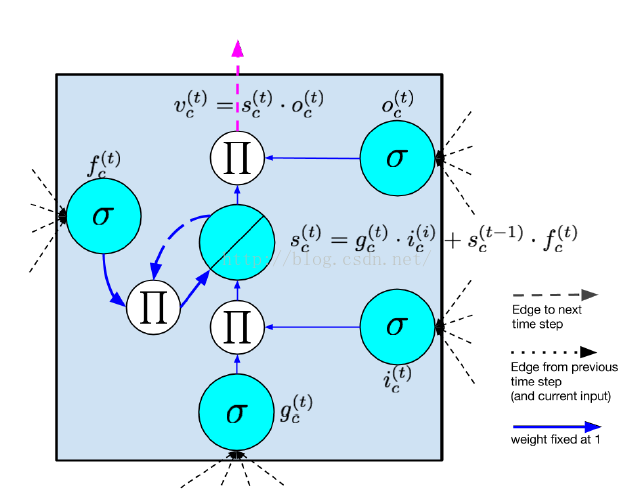
\includegraphics[width=0.6\textwidth]{lstmCell}
	\caption[Một "LSTM cell"]{Mô hình RNN đơn giản với kết nối vòng, \textbf{$h$} được xem như bộ nhớ được luân chuyển trong RNN. Chú ý rằng đường nét đứt ở đầu ra thể hiện rằng tại một thời điểm $t$, RNN có thể có hoặc không có một đầu ra.}
	\label{fig_lstmCell}
\end{figure}

Hochreiter và Schmidhuber \cite{hochreiter1997} đã giới thiệu mô hình \textit{Long short-term memory} (LSTM) chủ yếu ở để khắc phục vấn đề biến mất gradient trong RNN. Nhớ lại rằng trong RNN, chính việc mô hình hóa phụ thuộc thời gian dựa vào ma trận trọng số $W_{hh}$ đã gây ra hiện tượng gradient biến mất. Ý tưởng của LSTM là thay vì tính toán $h_t$ từ $h_{t-1}$ với một phép nhân ma trận theo sau là hàm kích hoạt phi tuyến, LSTM trực tiếp tính toán một $\Delta h_t$ sau đó nó được cộng với $h_{t-1}$ để tạo ra $h_t$. Thoạt nhìn, sự khác biệt này có thể không đáng kể khi mà chúng ta đều đạt được $h_t$ trong cả hai cách. Tuy nhiên, với cách làm này, gradient của $\Delta h_t$ sẽ không bị biến mất.

Thuật ngữ "Long short-term memory" xuất phát từ nhận định sau. Mạng RNN đơn giản có "long term memory" (bộ nhớ dài hạn) dưới dạng các ma trận trọng số. Những ma trận trọng số này thay đổi một cách chậm rãi trong quá trình học nhằm mã hóa kiến thức về dữ liệu. RNN cũng có "short-term memory" (bộ nhớ ngắn hạn) dưới dạng các kích hoạt tạm thời, được truyền từ mỗi bước thời gian sang các bước thời gian sau đó. "Long short-term memory" tạm dịch là "bộ nhớ ngắn hạn dài" cho phép mở rộng bộ nhớ ngắn hạn bằng cách thêm vào một loại lưu trữ trung gian gọi là trạng thái lưu giữ (cell state). Trạng thái lưu giữ này có khả năng lưu giữ các thông tin cần thiết một cách lâu dài dưới dạng một bộ nhớ ngắn hạn. Để làm được điều này, LSTM sử dụng một cơ chế gọi là "cổng", các "cổng" giúp được huấn luyện để chọn lọc thông tin nào là cần thiết để tác động lên trạng thái lưu trữ. Với cách làm này, trạng thái lưu trữ sẽ lưu được nhiều thông tin hơn, vì chỉ những thông tin quan trọng mới tồn tại trong nó.

Về cấu tạo, một LSTM tương tự như một RNN một lớp ẩn, nhưng mỗi "RNN cell" (ký hiệu "A" trong hình \ref{fig_rnn_unrolled}) được thay thế bằng một "memory cell" (hình \ref{fig_lstmCell}). Giống như "RNN cell", "memory cell" nhận một đầu vào bên ngoài và phát sinh một đầu ra cũng như là truyền đi một trạng thái ẩn sang "memory cell" ở bước thời gian kế tiếp. Tuy nhiên, trong "memory cell" còn có thêm một trạng thái lưu giữ cũng được truyền đi như một trạng thái ẩn. Cấu tạo chi tiết của LSTM sẽ được trình bày trong phần dưới đây, cấu tạo này dựa trên phiên bản LSTM của \cite{Gers2000}.

\begin{itemize}
	\item[•] \textit{Nút đầu vào (input node)}: Đơn vị này được ký hiệu là $g$, là một mạng nơ-ron một tầng ẩn. Nút đầu vào có nhiệm vụ mô hình hóa đầu vào tại mỗi bước thời gian. Nó nhận tham số là đầu vào tại bước thời gian hiện tại $x_t$ và trạng thái ẩn tại thời điểm trước đó $h_{t-1}$. Cụ thể, tại mỗi bước thời gian nút đầu vào có công thức:
	\begin{equation} \label{inputNodeLSTM}
		g_t = \phi \left(W_{gx}x_t + W_{gh}h_{t-1} + b_g \right)
	\end{equation}
	\item[•] \textit{Cổng vào (input gate)}: "Cổng" như đã nói, là một cơ chế đặc biệt của LSTM. Cổng vào cũng được cấu tạo giống như nút đầu vào, nó nhận tham số là $x_t$ và $h_{t-1}$. Sau đó được đưa qua hàm kích hoạt $\sigmoid$ để tạo ra giá trị trong khoảng $(0,1)$. Sở dĩ đơn vị này được gọi là "cổng vào" vì giá trị của nó sẽ được sử dụng để nhân với giá trị của nút đầu vào. Giá trị của nó thể hiện lượng thông tin mà nút đầu vào được phép truyền đi. Nếu cổng vào bằng 0, nút đầu vào sẽ truyền đi với giá trị 0. Nếu cổng vào bằng 1, nút đầu vào sẽ truyền đi với giá trị ban đầu. Cụ thể hơn, ta có công thức của cổng vào, được ký hiệu là $i$, tại bước thời gian $t$:
	\begin{equation} \label{inputGateLSTM}
		i_t = \sigma \left(W_{ix}x_t + W_{ih}h_{t-1} + b_i \right)
	\end{equation}
	\item[•] \textit{Trạng thái lưu giữ (cell state)}: Trái tim của LSTM chính là trạng thái lưu trữ, là một mạng nơ-ron với hàm kích hoạt tuyến tính. Khá giống với trạng thái ẩn trong RNN, trạng thái lưu trữ $s_t$ cũng có một kết nối hồi quy với trạng thái lưu trữ trước đó $s_{t-1}$. Tuy nhiên, trọng số kết nối hồi quy luôn có giá trị cố định là 1. Bởi vì kết nối hồi quy này qua nhiều bước đều có trọng số không đổi nên khi tính toán, "gradient" của độ lỗi không bị bùng nổ hay biến mất. Tại mỗi bước thời gian, trạng thái lưu trữ được tính như sau:
	\begin{equation} \label{cellStateLSTM}
		s_t = s_{t-1} + g_t \odot i_t
	\end{equation}
	\item[•] \textit{Cổng quên (forget gate)}: Là trái tim của LSTM. Cổng quên là một đề xuất của \cite{Gers2000} so với bài báo LSTM gốc. Thay vì kiểm soát lượng thông tin để đưa vào trạng thái lưu giữ như cổng vào, cổng quên cung cấp khả năng tẩy đi một lượng thông tin trong trạng thái lưu giữ. Cụ thể, cổng quên với giá trị thuộc khoảng $(0,1)$ sẽ được nhân với $s_{t-1}$ trong công thức \ref{cellStateLSTM}. Tại mỗi bước thời gian, giá trị của cổng quên $f_t$ được tính như sau:
	\begin{equation} \label{forgetGateLSTM}
		f_t = \sigma \left(W_{fx}x_t + W_{fh}h_{t-1} + b_f \right)
	\end{equation}
	Công thức của trạng thái lưu trữ được sửa lại khi có cổng quên:
	\begin{equation} \label{cellStateWithForgetGateLSTM}
		s_t = s_{t-1} \odot f_t + g_t \odot i_t
	\end{equation}
	\item[•] \textit{Cổng ra (output gate)}:
\end{itemize}



\section{Mô hình ngôn ngữ}

Như chúng tôi đã đề cập trong chương 1, \textit{mô hình ngôn ngữ} (language model) là một bộ phận quan trọng trong cả dịch máy thống kê và dịch máy nơ-ron. Cụ thể hơn, mô hình ngôn ngữ là một phân phối xác suất trên một chuỗi các từ. Cho trước một chuỗi $w_1,w_2,...,w_m$ (ký hiệu $w_{1:n}$), mô hình ngôn ngữ gán cho nó một xác suất $P(w_{1:n})$ đại diện cho độ "trơn tru" của chuỗi đó. Sử dụng quy tắc dây chuyền (chain rule) trong xác suất, ta có:
\begin{equation} \label{lmGeneral}
	P(w_{1:n}) = P(w_1)P(w_2|w_1)P(w_3|w_{1:2})P(w_4|w_{1:3})...P(w_n|w_{1:n-1})
\end{equation}














